\institute{Universite Paris-Sud / CEA Saclay}

\title{Data-driven correction of electromagnetic shower shapes in Monte-Carlo modelling of ATLAS calorimeter}


\author{Mykola Khandoga}

\maketitle
\begin{abstract}
The electromagnetic calorimeter is one of the key elements of the ATLAS detector at the Large Hadron Collider at CERN. 
In order to properly reconstruct the physical processes happening after the collision it is crucial to identify the origin of the measured particles and, in particular, to separate the signal electrons, coming from prompt decays, from the background. 
Electron identification is performed by means of multi-variant analysis algorithm, which in turn strongly relies on a number of electromagnetic shower shape characteristics. \\
The Monte-Carlo model provides inaccurate energy distribution in the calorimeter cluster cells.
Correcting the shower shapes allows to improve the electron identification and decrease the associated systematic uncertainty.
\end{abstract}

\section{Introduction}

The ATLAS calorimeter is a very important part of the detector and consists of electromagnetic and hadronica part. The former is designed to provide precision measurements of electrons, photons and jets energy as well as the missing transverse energy. Aside from energy measurements information from the calorimeter is also used for particle identification (ID). Particle ID, in turn, is crucial for most of the physics analysis in ATLAS. Hereafter we use the ATLAS coordinate system where z axis is directed along the beam, $\phi$ is the asimutal angle along the beam pipe, pseudorapidity $\eta =  −ln[tan (\theta/2)]$, where $\theta$ is the polar angle.  Transverse momentum and energy are defined as $p_T =$ p $sin\theta$, $E_T =$E $sin\theta$ respectively.

\begin{figure}[htbp]
 \begin{center}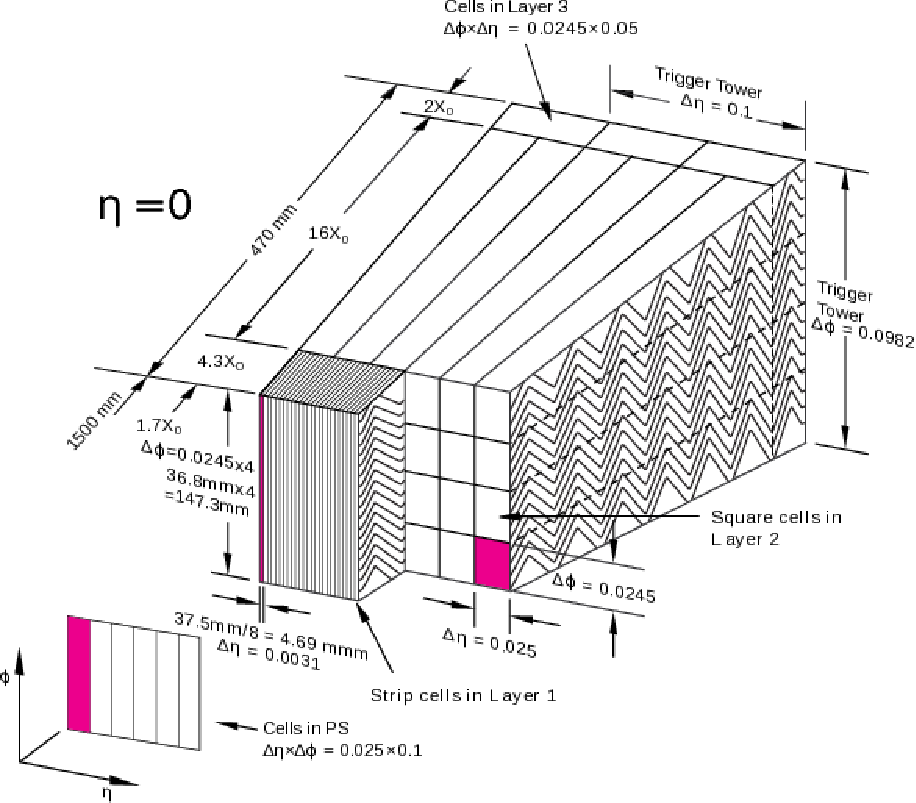
\includegraphics[%
  width=7cm,
  keepaspectratio]{Calo_cells.pdf}
 \end{center}
\caption{Layout of the ATLAS electromagnetic calorimeter.}
\label{calocells}
\end{figure}
ATLAS electromagnetic calorimeter \ref{TDR} consists of three layers and a pre-sampler. The first layer has very high granularity in $\eta$ dimension. The second layer has high granularity in both $\eta$ and $\phi$ dimensions and also absorbs most of the energy of electrons and photons. Such a fine structure of the detector not only allows to perform a precise measurement of particle energy but also to observe the development of the electromagnetic shower in all three dimensions. \\
A number of variables called shower shapes are used to describe shower development in different layers of the calorimeter and then are used as an input for particle identification MVA algorithm.\\
Current study primarily concentrates on the variables obtained from the second layer of the calorimeter, considering their importance for the MVA:
\begin{itemize}
\item Lateral shower width $W_{\eta^2} = \sqrt{\sum(E_i \eta^{2}_{i})-(\sum(E_i \eta_{i})/\sum(E_i))^2}$ calculated within a window of 3x5 cells ($\eta x \phi$).
\item $R_{\phi}$ - ratio of the energy in 3x3 cells over the energy in 3x7 cells centered at the electron cluster position.
\item $R_{\eta}$ - ratio of the energy in 3x7 cells over the energy in 7x7 cells centered at the electron cluster position.
\end{itemize}
Figure \ref{Reta_simul} shows how $R_{\eta}$ distribution is different in jets, signal electrons and background electrons. Background electrons denot non-prompt electrons which are not originated from primary vertex.\\
\begin{figure}[htbp]
 \begin{center}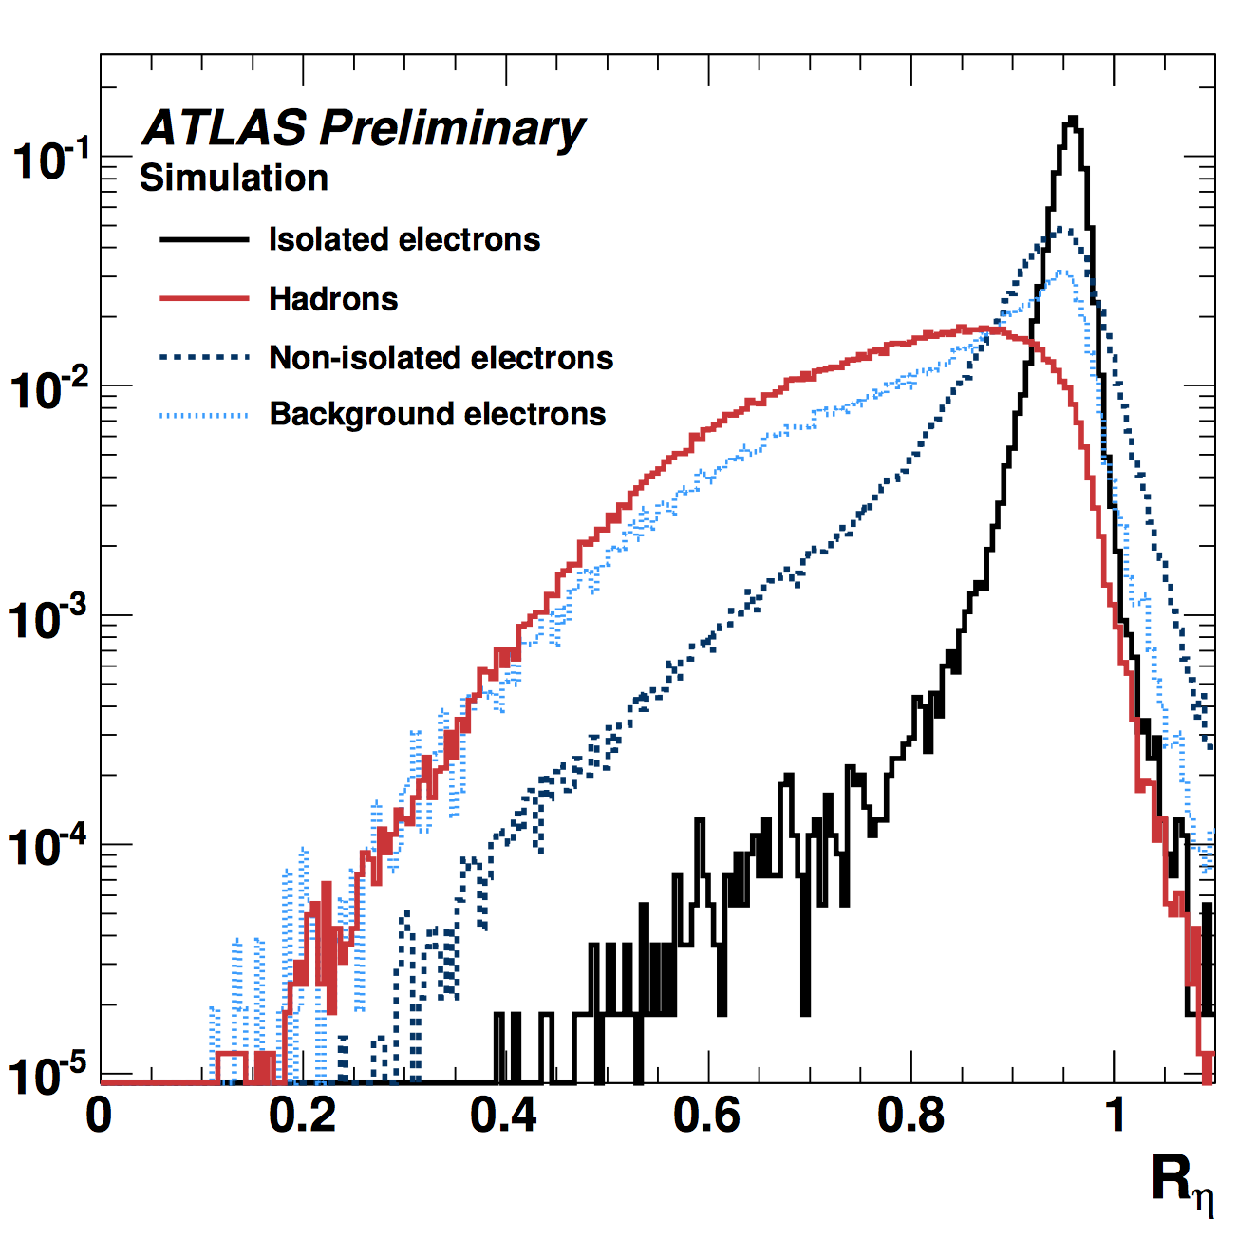
\includegraphics[%
  width=7cm,
  keepaspectratio]{RetaSimulation.pdf}\\
 \end{center}
\caption{Distribution of $R_{\eta}$ in simulation (GEANT4) for electrons and jets}
\label{Reta_simul}
\end{figure}
\\
The shower shapes-based approach has proven to be a reliable source of information but also revealed a number of discrepancies between the data and MC (Powheg+Pythia8+GEANT4) modelling. This, in turn, leads to discrepancies in particle ID which are later corrected using highly $\eta-$ and $p_T$-dependent scale factors. 
The actual origin of the discrepancy is not clear.  \\
Correction of the shower shapes aims to get the scale factors closer to unity, reducing the corresponding systematic uncertainties and improving the precision of the measurements with electrons in the final states.  
% La figure~\ref{PortraitRabelais} repr{\'e}sente Fran{\c c}ois Rabelais. %
%\begin{figure}[htbp]
%\begin{center}\includegraphics[%
%  width=2.5cm,height=5cm]{A.eps}
  %keepaspectratio
%\end{center}

%\caption{\label{fig1} legende}
%\end{figure}%

%Ceci est une boule \ref{boule}, donnant des recommandations et des
%exemples pour une contribution aux RJC2006.

\section{ Shower shapes measurement and correction  }
\subsection{Event selection}
For this study we have considered electrons from the $Z\rightarrow ee$ decay. A set of recommended single electron triggers was used. Each event was required to have 2 electrons at least one of which has $p_T>25$GeV.  In order to suppress the background both electrons had to pass gradient isolation. Z invariant mass cut was applied with a window of $80-120$GeV. To avoid identification bias from triggering the tag and probe approach was used with only probe electrons taken into consideration \ref{RecoID2011}. The electron cluster in the second calorimeter layer was required to contain information from 77 calorimeter cells. Datasets of $10^7$ events in data (2017 proton-proton collisions) and $7*10^6$ events in MC (Powheg+Pythia8) were used.
\subsection{Data/MC discrepancies}
Our consideration begins with the energy deposit of an electron in the second layer of the calorimeter. A window of 7 cells in $\eta$ and 11 cells in $\phi$ is centered around the cell with the highest energy.
\begin{figure}[htbp]
\begin{center}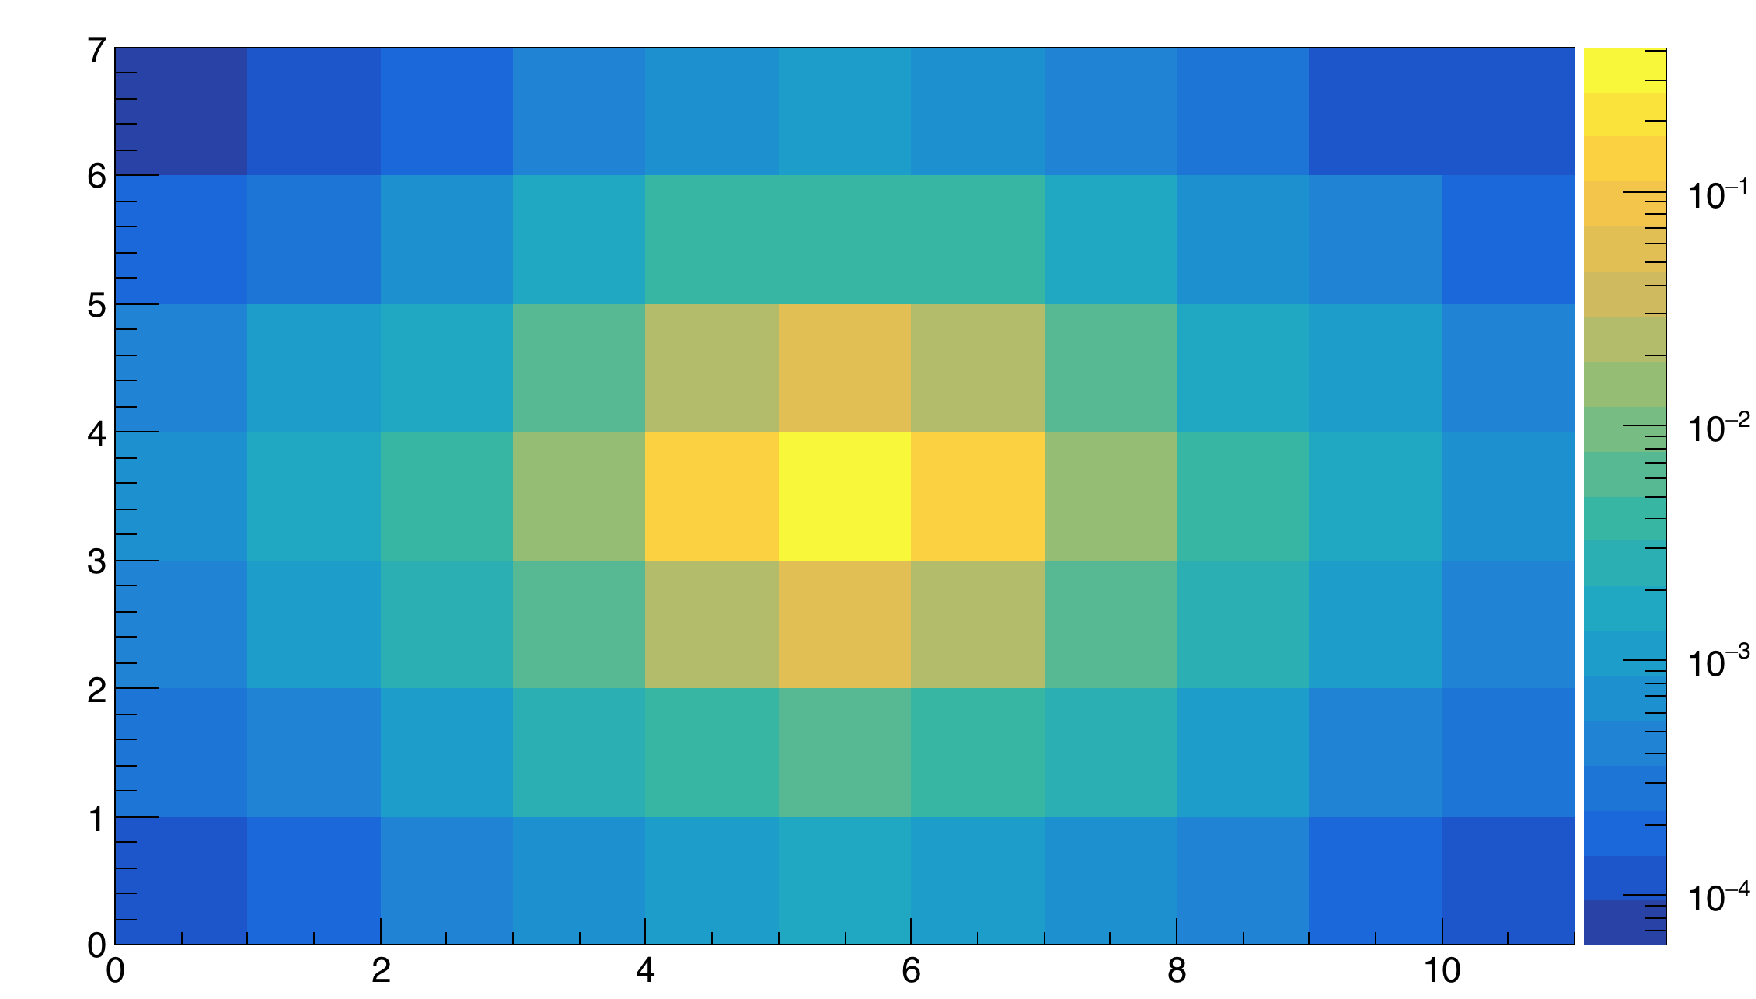
\includegraphics[%
  width=7cm,
  keepaspectratio]{logscale.pdf}\end{center}
\caption{Energy profile of a window of 7x11 cells in the 2nd calorimeter layer (logarithmic scale) }
\label{2dprofile}
\end{figure}
Shower shapes were considered in 14 $\eta$ bins in the range between $|\eta| = (0,2.4)$ in order to investigate how the discrepancy depends on $\eta$. 

\begin{figure}[htbp]
\begin{center}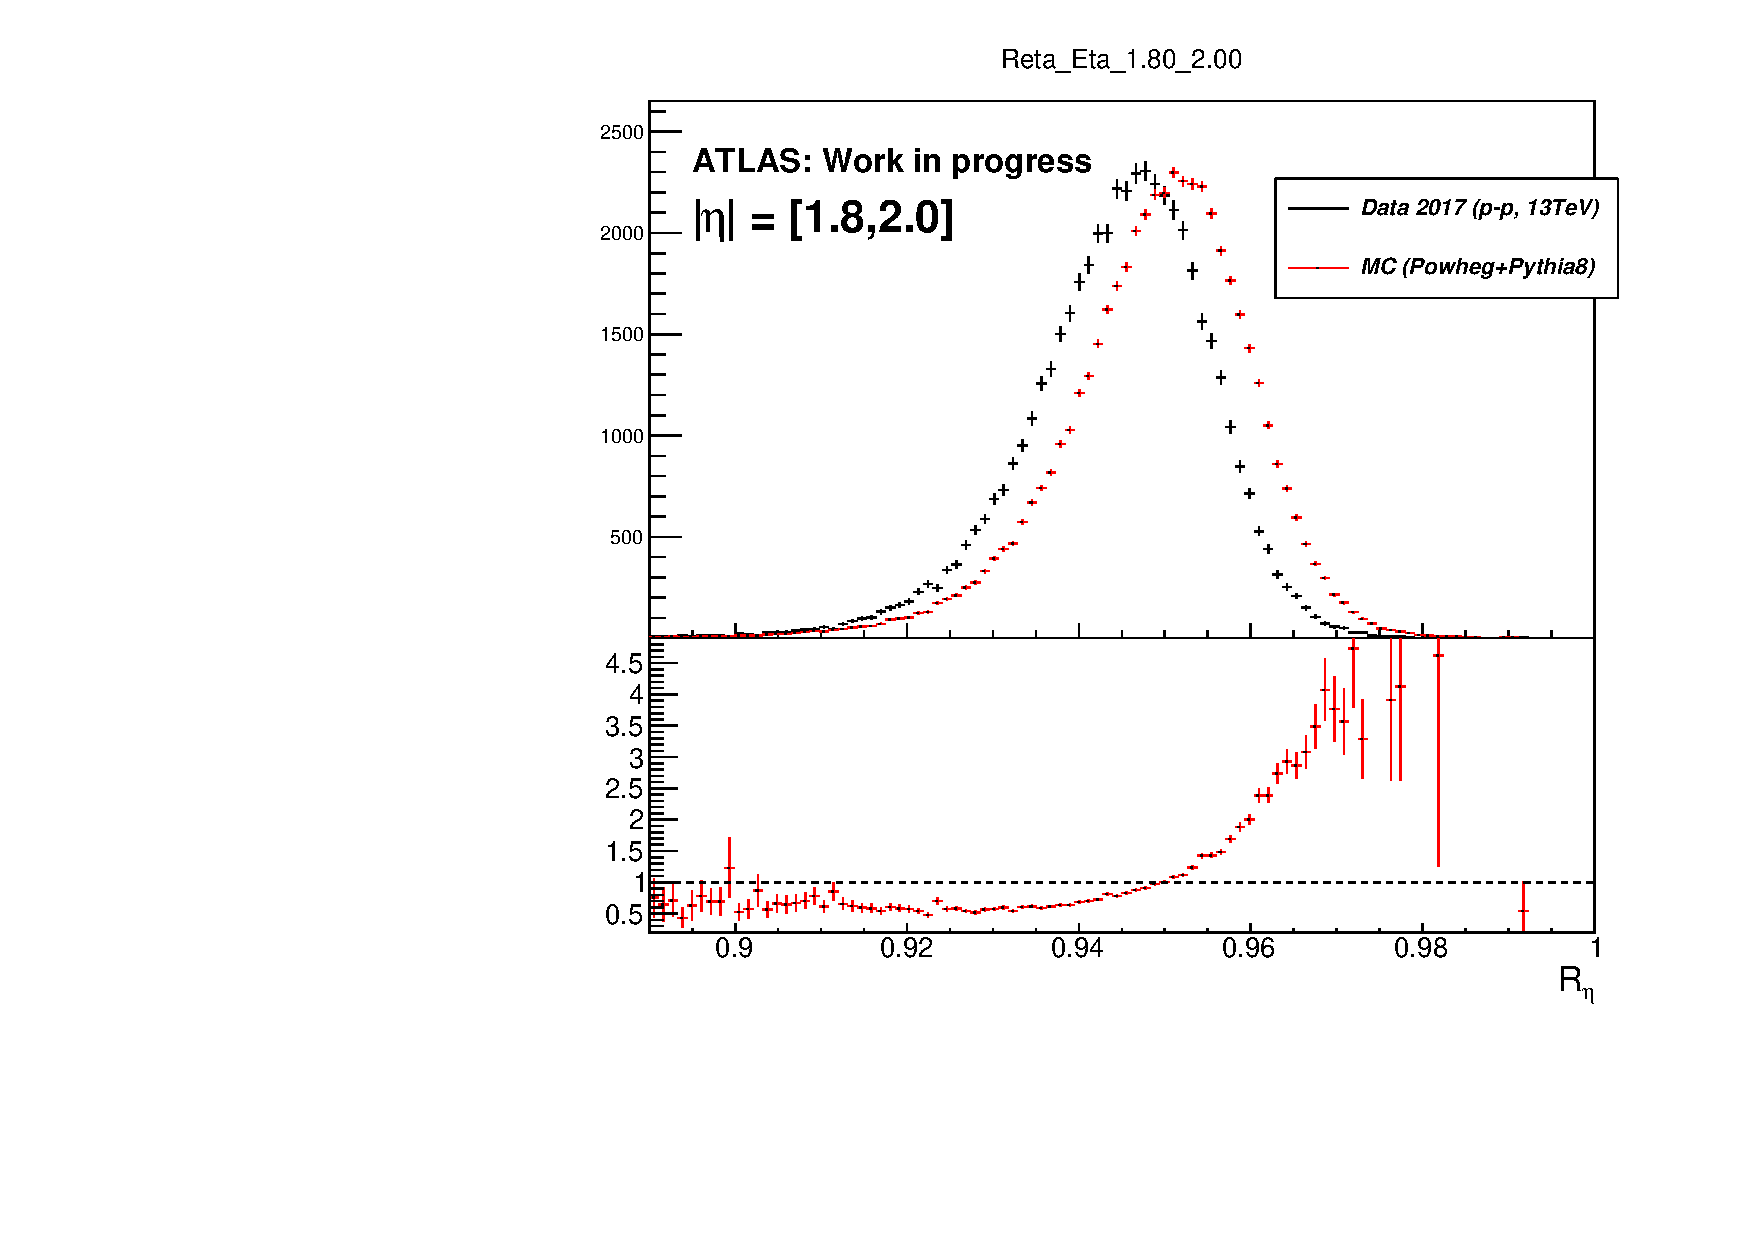
\includegraphics[%
  width=7cm,
  keepaspectratio]{Reta2_Eta_18_20.pdf}\end{center}
\caption{$R_{\eta}$ in $|\eta| = (1.8,2.0)$ }
\label{Reta2}
\end{figure}
\begin{figure}[htbp]
\begin{center}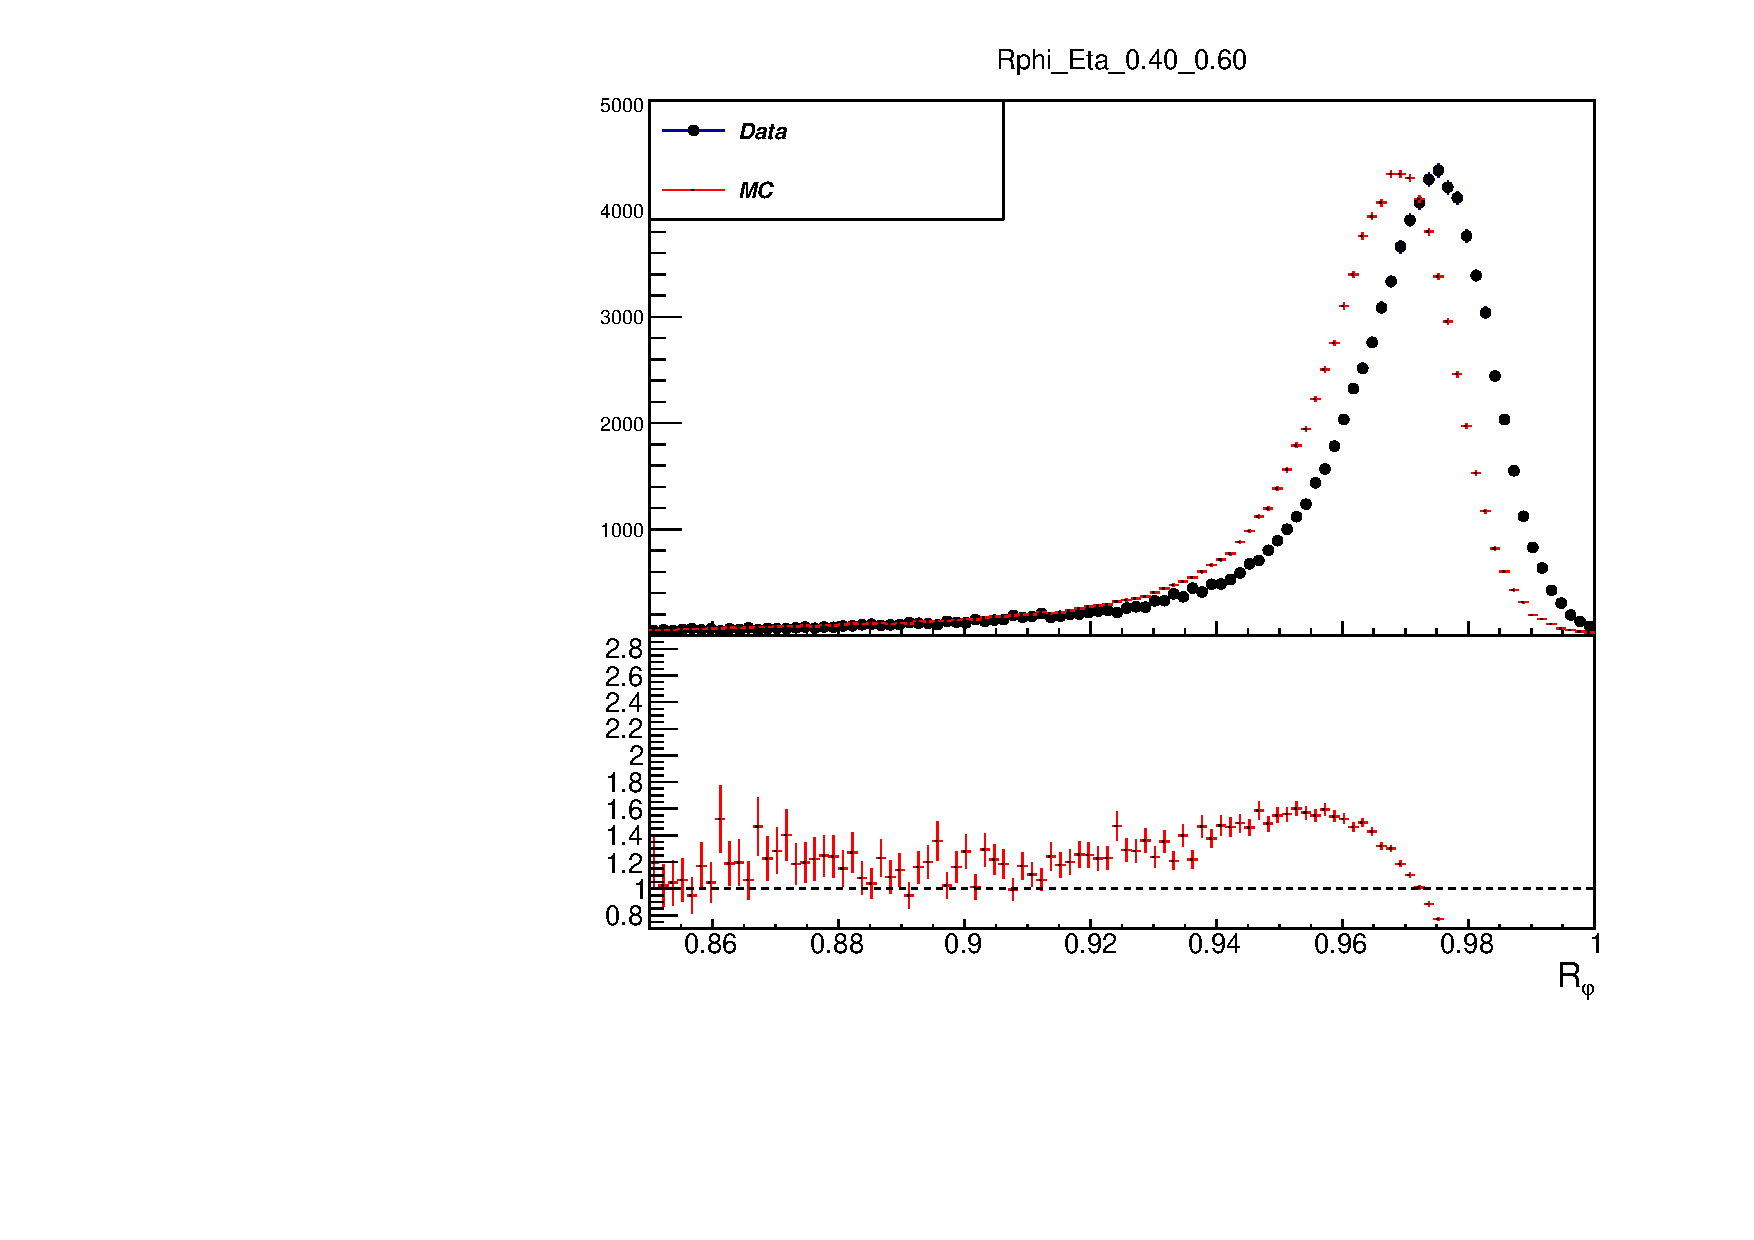
\includegraphics[%
  width=7cm,
  keepaspectratio]{Rphi2_Eta_4_6.pdf}\end{center}
\caption{$R_{\phi}$ in $|\eta| = (0.4,0.6)$ }
\label{Rphi2}
\end{figure}
\begin{figure}[htbp]
\begin{center}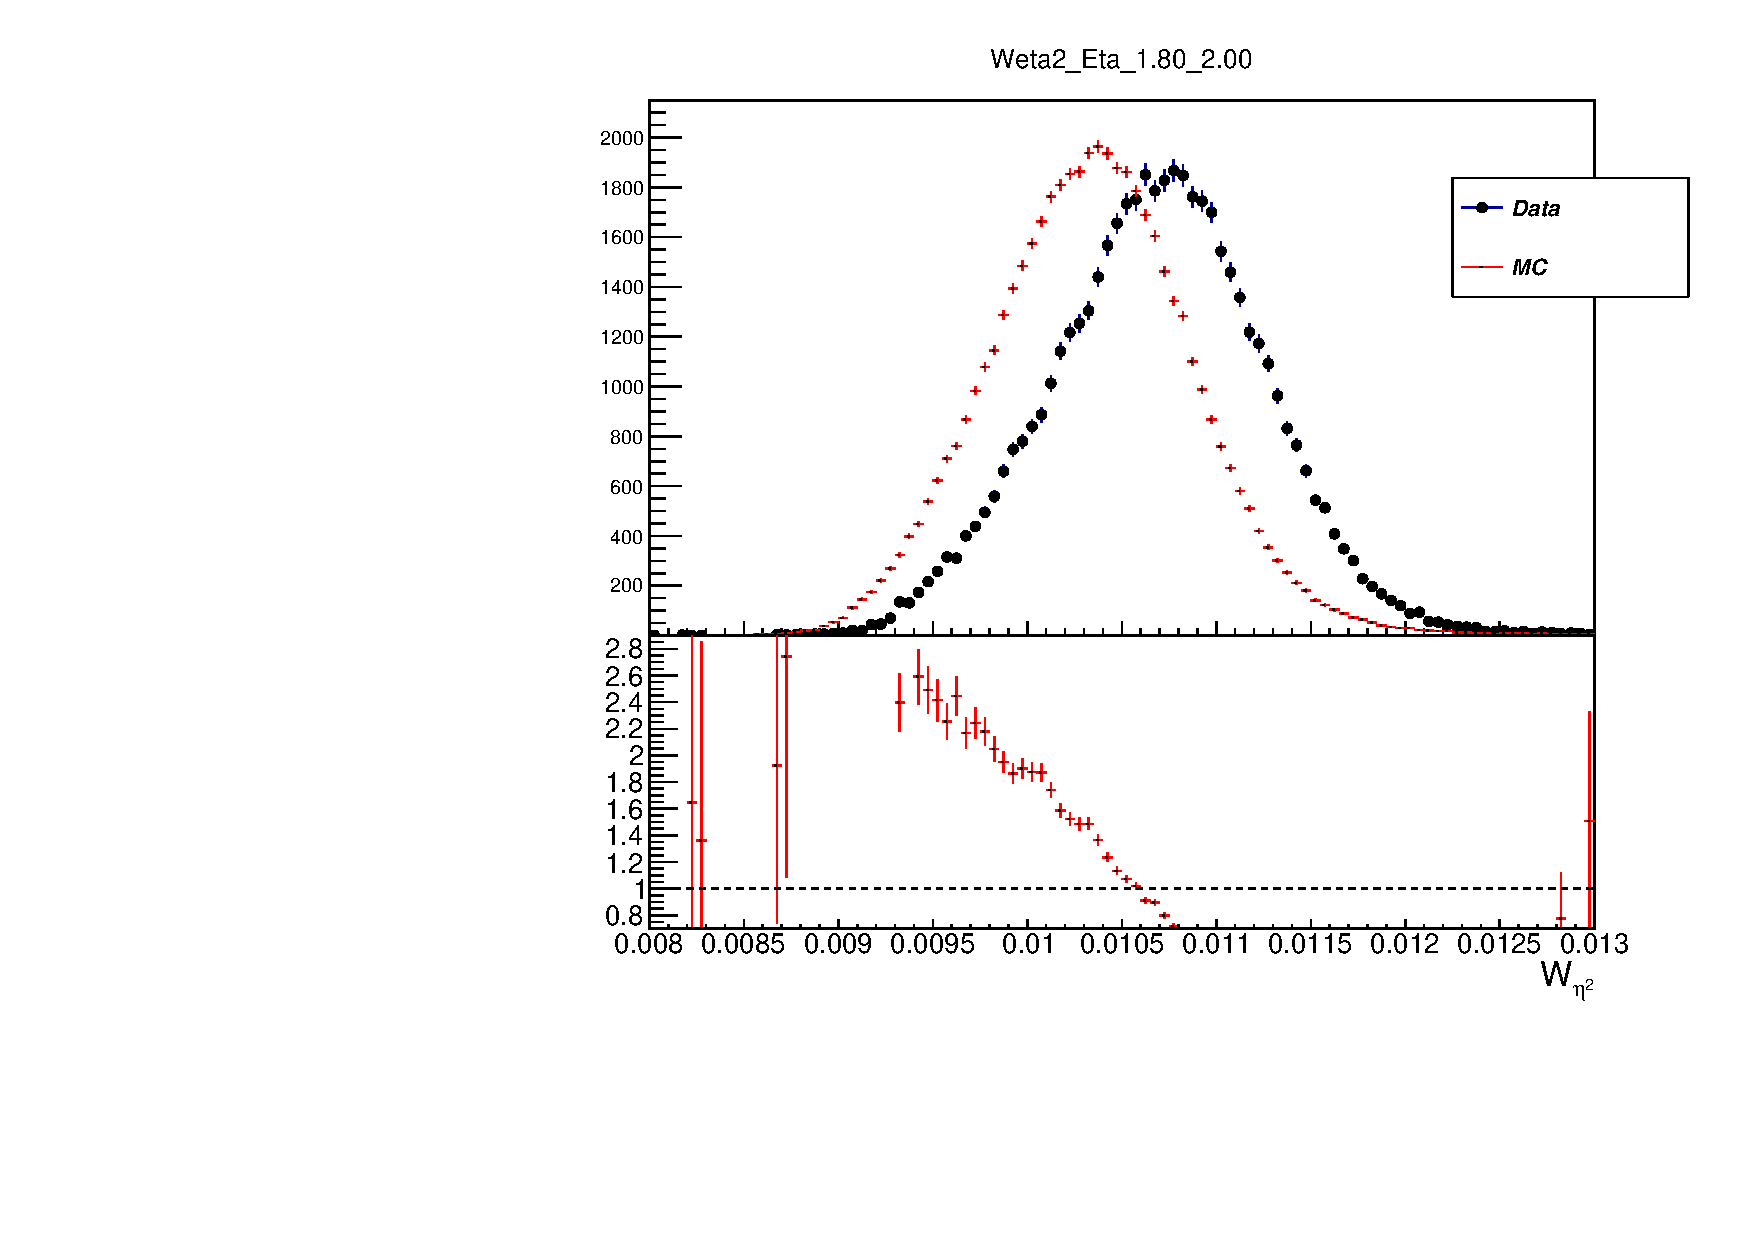
\includegraphics[%
  width=7cm,
  keepaspectratio]{weta22_Eta_18_20.pdf}\end{center}
\caption{$W_{\eta 2}$ in $|\eta| = (1.8,2.0)$  }
\label{Weta22}
\end{figure}

\\
The $\eta$-dependent shower shapes in data are wider than the MC and show a larger discrepancy in the endcap ($|\eta| = (1.52,2.4)$). For $\phi$ dimension the situation is the opposite: MC is wider than the data and the barrel ($|\eta| = (0,1.52)$) shows larger discrepancy. Figures \ref{Reta2}, \ref{Rphi2}, \ref{Weta22} contain examples of shower shapes in different eta bins. 
 \subsection{The correction procedure}
 \subsubsection{The correction matrix}
The correction procedure is based on the redistribution of energy between the cluster cells in MC so that the distribution becomes consistent with the data. For every $\eta$ bin a correction matrix is derived in the following way:
\begin{equation}
\nonumber
   \large {M_{i}^{Correction} = \frac{E_{i}^{Data}}{\Sigma E^{Data}} - \frac{E_{i}^{MC}}{\Sigma E^{MC}}}
\end{equation}
$\Sigma_i M_i^{Correction} = 0$, $i = 1..77$.\\
$E_i^{Data}$, $E_i^{MC}$ - matrix elements of the averaged energy profiles. 
The correction is then applied to the electron cluster cells on event-by-event basis:
\begin{equation}
\nonumber
   \large {E_{i}^{Reweighted} = {E_{i}^{Non-reweighted}(1+M_{i}^{Correction}).}}
\end{equation}
This redistributes the energy among the cells keeping the total energy exactly the same.
 \subsubsection{Bremsstrahlung tails}
The magnetic field directed along the $\phi$ dimension leads to a significant asymmetry in energy deposits for electrons and positrons (figure \ref{chargeAsym}). 
\begin{figure}[htbp]
\begin{center}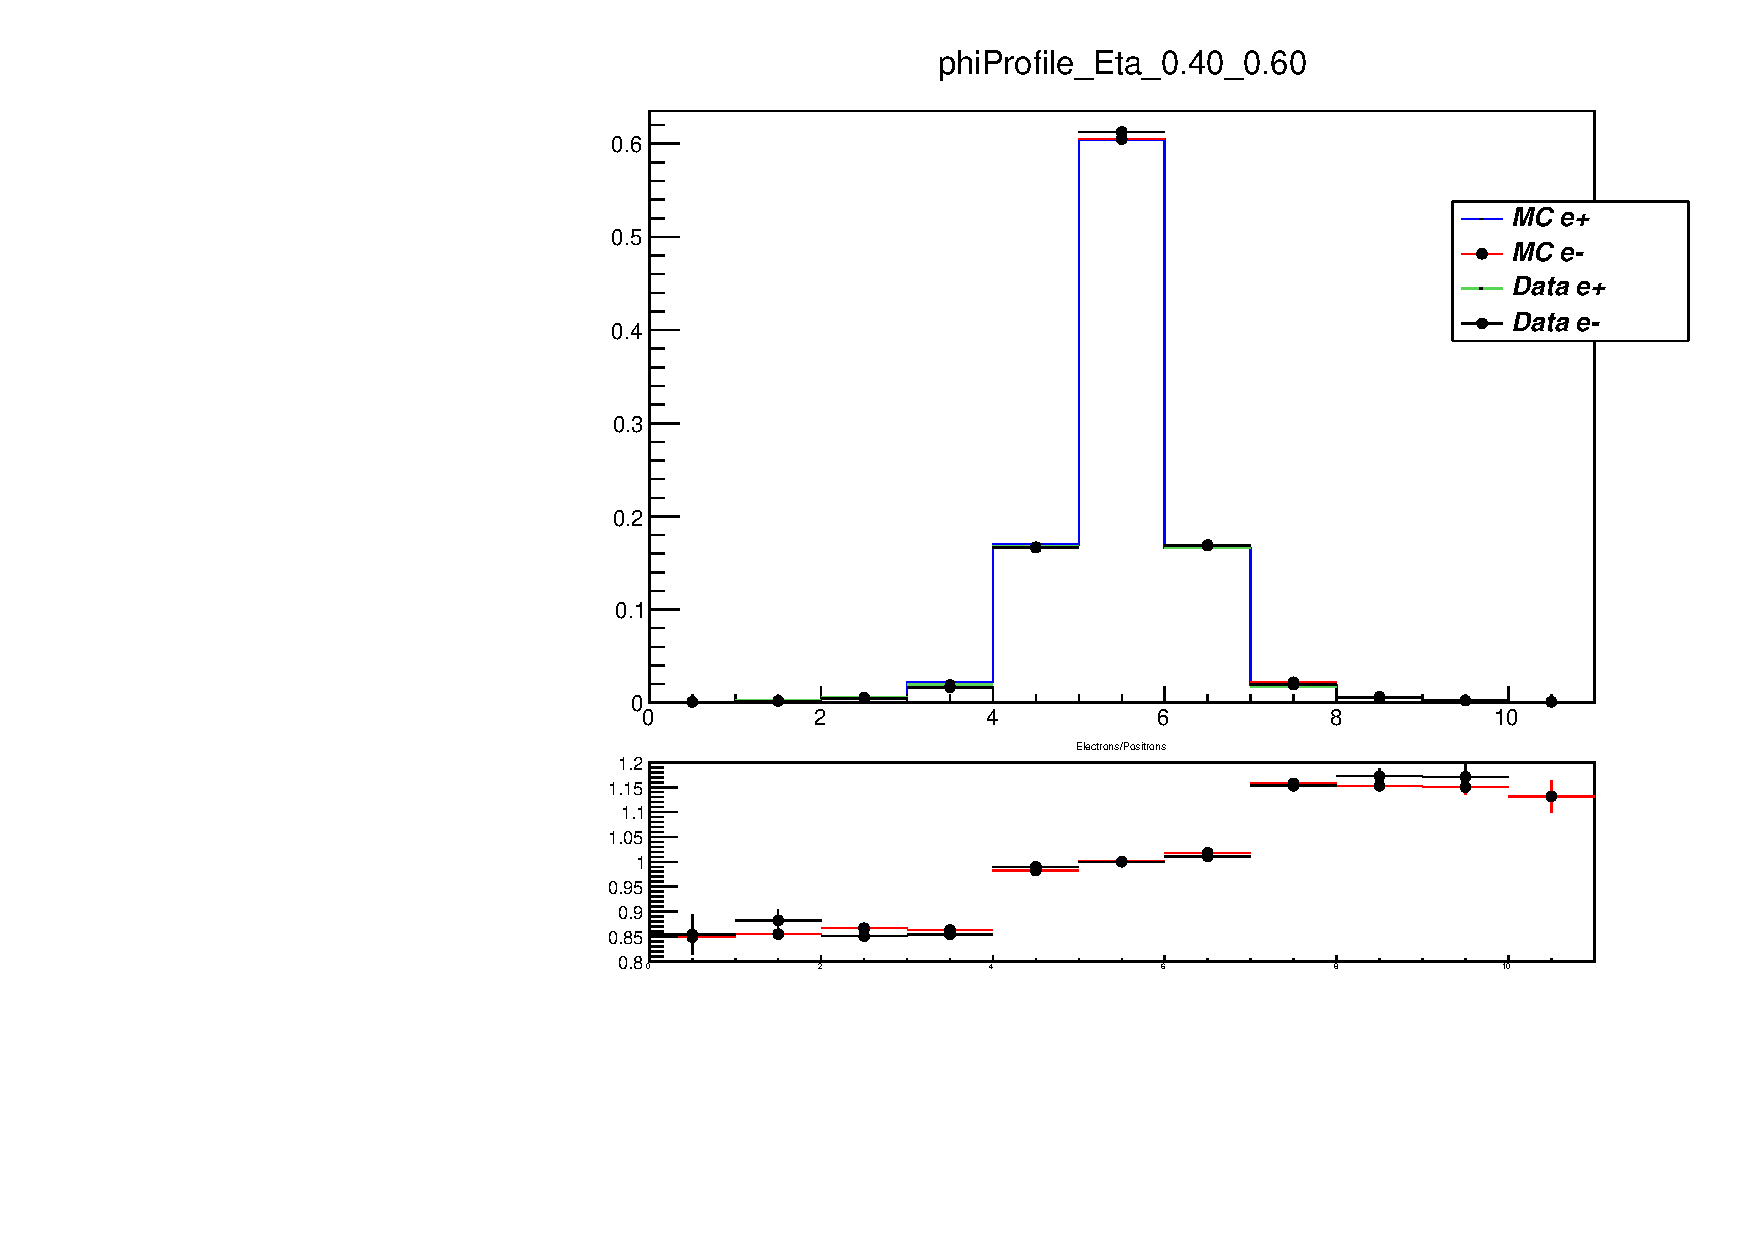
\includegraphics[%
  width=7cm,
  keepaspectratio]{phiProfileDataMC_Eta_4_6.pdf}\end{center}
\caption{Energy profile in $\phi$ for $e^+$ and $e^-$. }
\label{chargeAsym}
\end{figure}
Considering the fact that the reweighting is intended to correct for the data/MC discrepancies themselves and not for the bremsstrahlung effect it makes sense to develop the bremsstrahlung-free correction function based on $e^+$ and $e^-$ correction matrices. The principle is schematically explained on figure \ref{bstails}.\\
\begin{figure}[htbp]
\begin{center}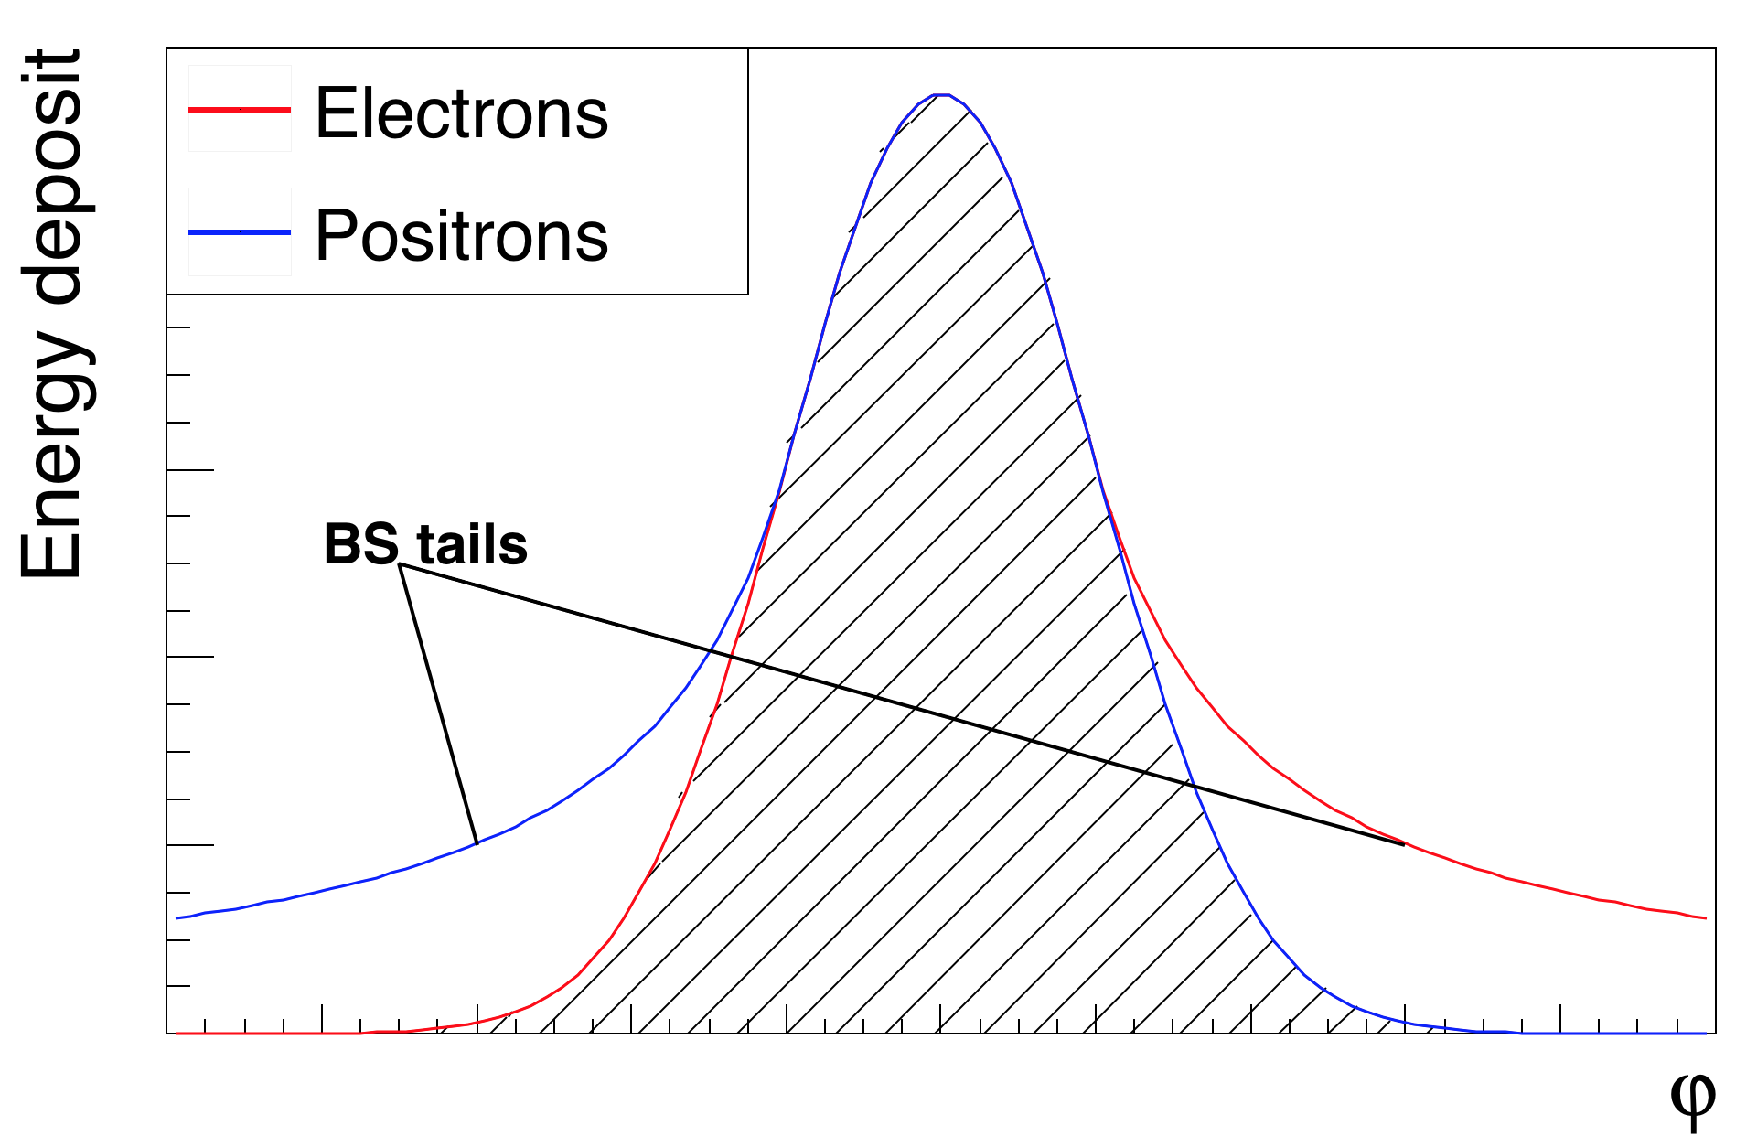
\includegraphics[%
  width=7cm,
  keepaspectratio]{bs_tails.pdf}\end{center}
\caption{Schematic energy profile in $\phi$ dimension. Bremsstrahlung tails subtraction based on $e^+$ and $e^-$ energy profiles.}
\label{bstails}
\end{figure}
Good agreement of data and MC description of $e^+$ and $e^-$ asymmetry gives a hint that the material mismodelling cannot be the main source of the data/MC disagreement.\\

\section{R\'esultats}
Figures \ref{Reta_reweighted}, \ref{Rphi_reweighted}, \ref{Weta_reweighted} show the effect of the correction. The shower shapes in MC become very close to the data, correcting a significant discrepancy. \\
Figures \ref{Rphi_vs_pT_Int}, \ref{Reta_vs_pT_Int}, \ref{Weta2_vs_pT_Int} contain shower shapes vs $p_T$ integrated over $\eta$. They demonstrate that the correction does not depend on the $p_T$ which allows to expect the decreased systematic uncertainties for $p_T$ regions distant from $40-50$GeV.\\
Finally, figure \ref{SF} shows the effect of the correction on electron ID efficiency. We can see a visible improvement, notably in the endcap region.
Nevertheless the barrel region shows little improvement. It can be explained by the fact that electron ID MVA relies on many variables while only a number of them were corrected during current study.\\
The proposed method is getting integrated into ATLAS Athena framework as an option and is planned to be used as a baseline for Run 3. 
\begin{figure}[htbp]
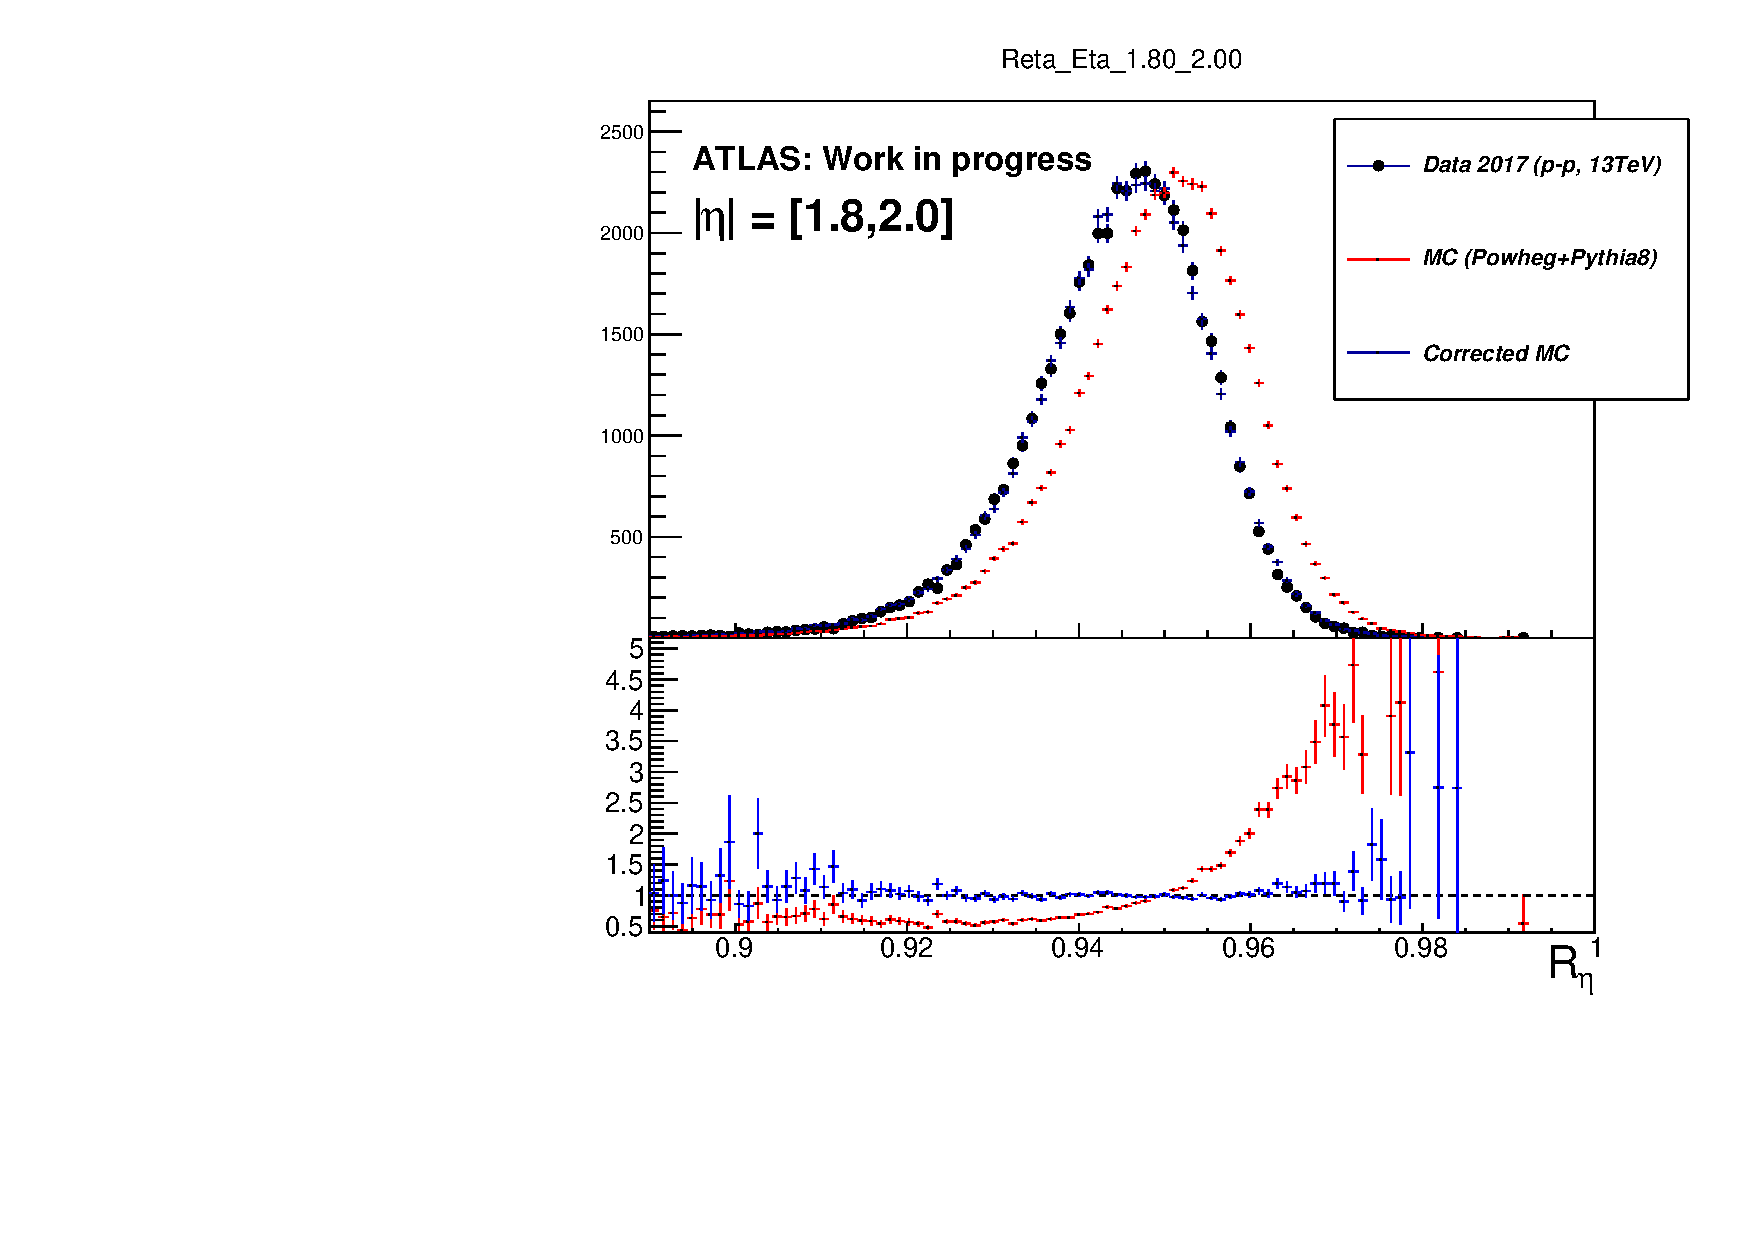
\includegraphics[%
  width=7cm,
  keepaspectratio]{Reta_Eta_18_20.pdf}
\caption{Reweighted  $R_{\eta }$ in $|\eta| = (1.8,2.0)$.  }
\label{Reta_reweighted}
\end{figure}

\begin{figure}[htbp]
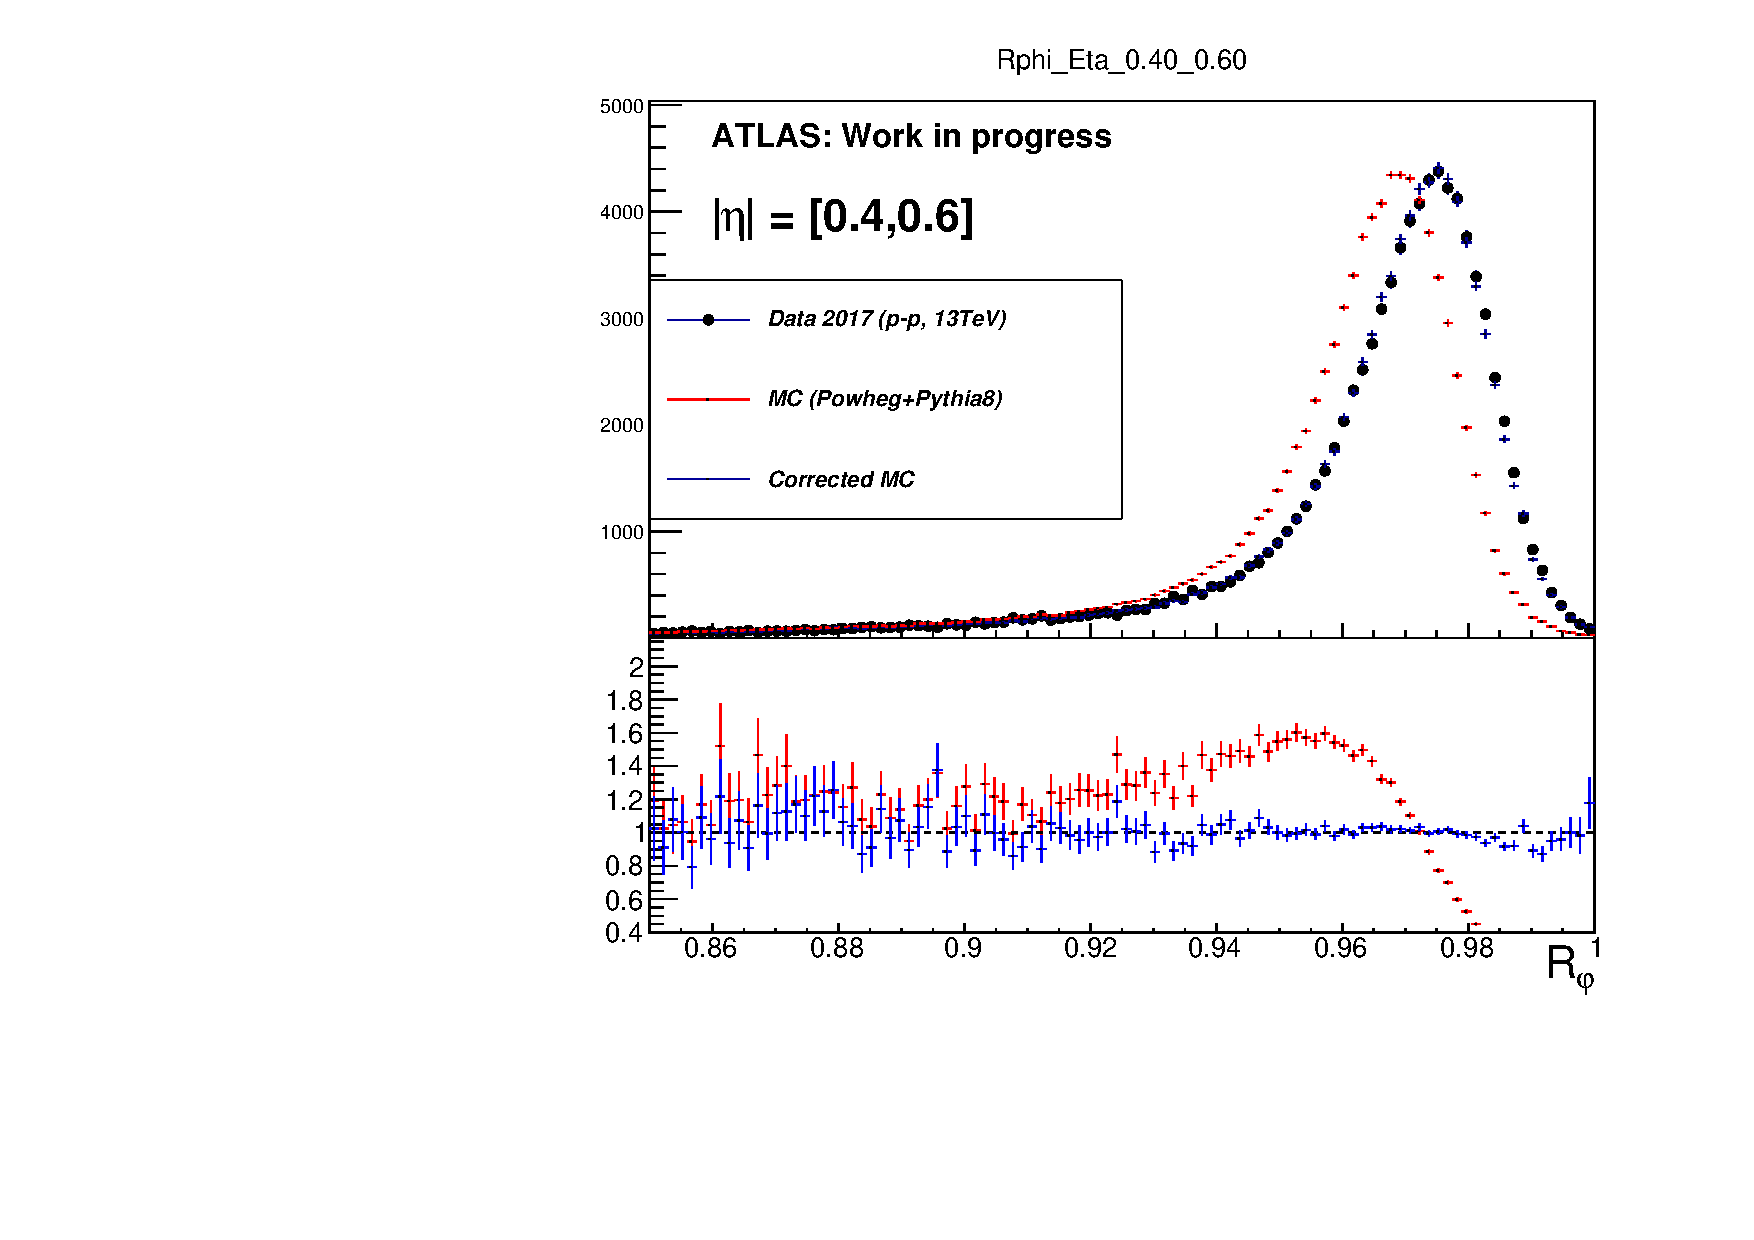
\includegraphics[%
  width=7cm,
  keepaspectratio]{Rphi_Eta_4_6.pdf}
\caption{Reweighted  $R_{\phi}$ in $|\eta| = (0.4,0.6)$.  }
\label{Rphi_reweighted}
\end{figure}

\begin{figure}[htbp]
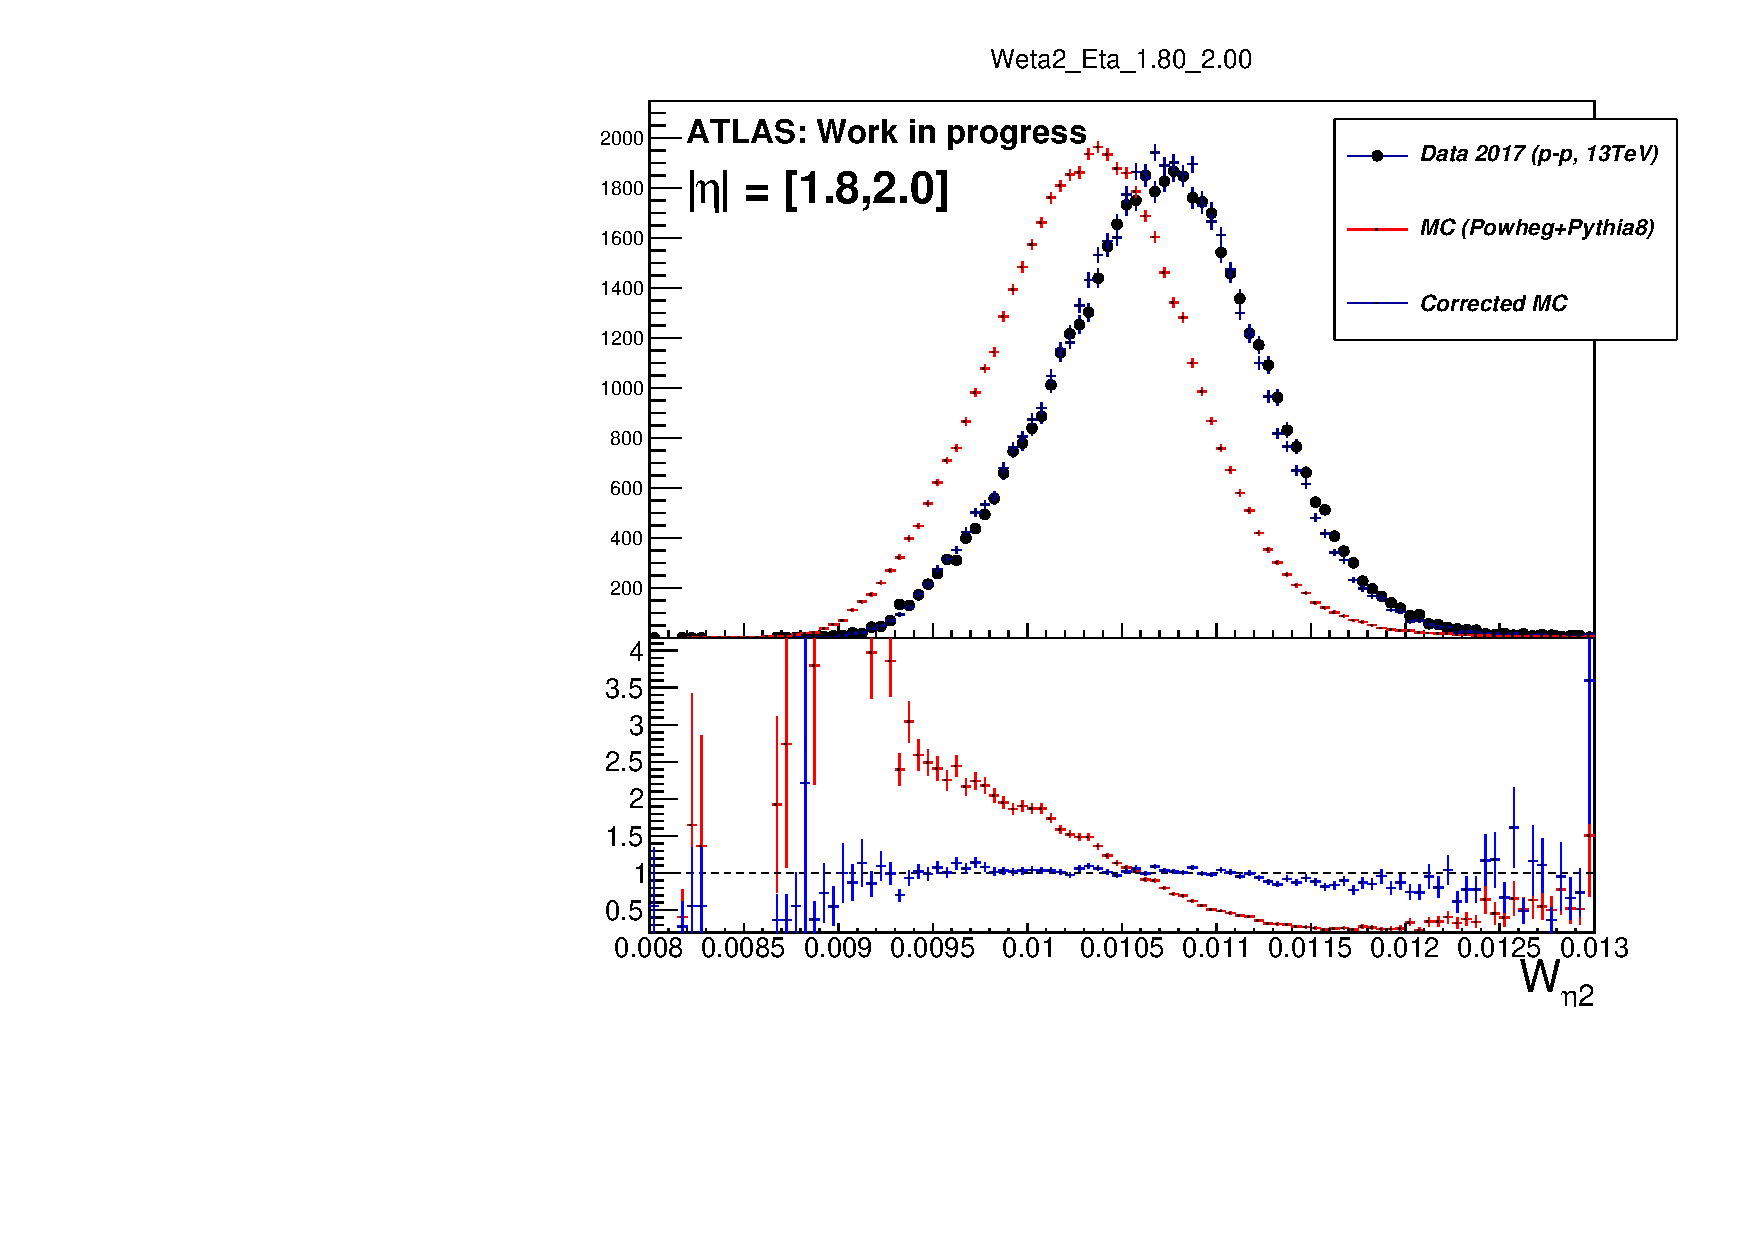
\includegraphics[%
  width=7cm,
  keepaspectratio]{Weta2_Eta_18_20.pdf}
\caption{Reweighted  $W_{\eta 2}$ in $|\eta| = (1.8,2.0)$.  }
\label{Weta_reweighted}
\end{figure}

\begin{figure}[htbp]
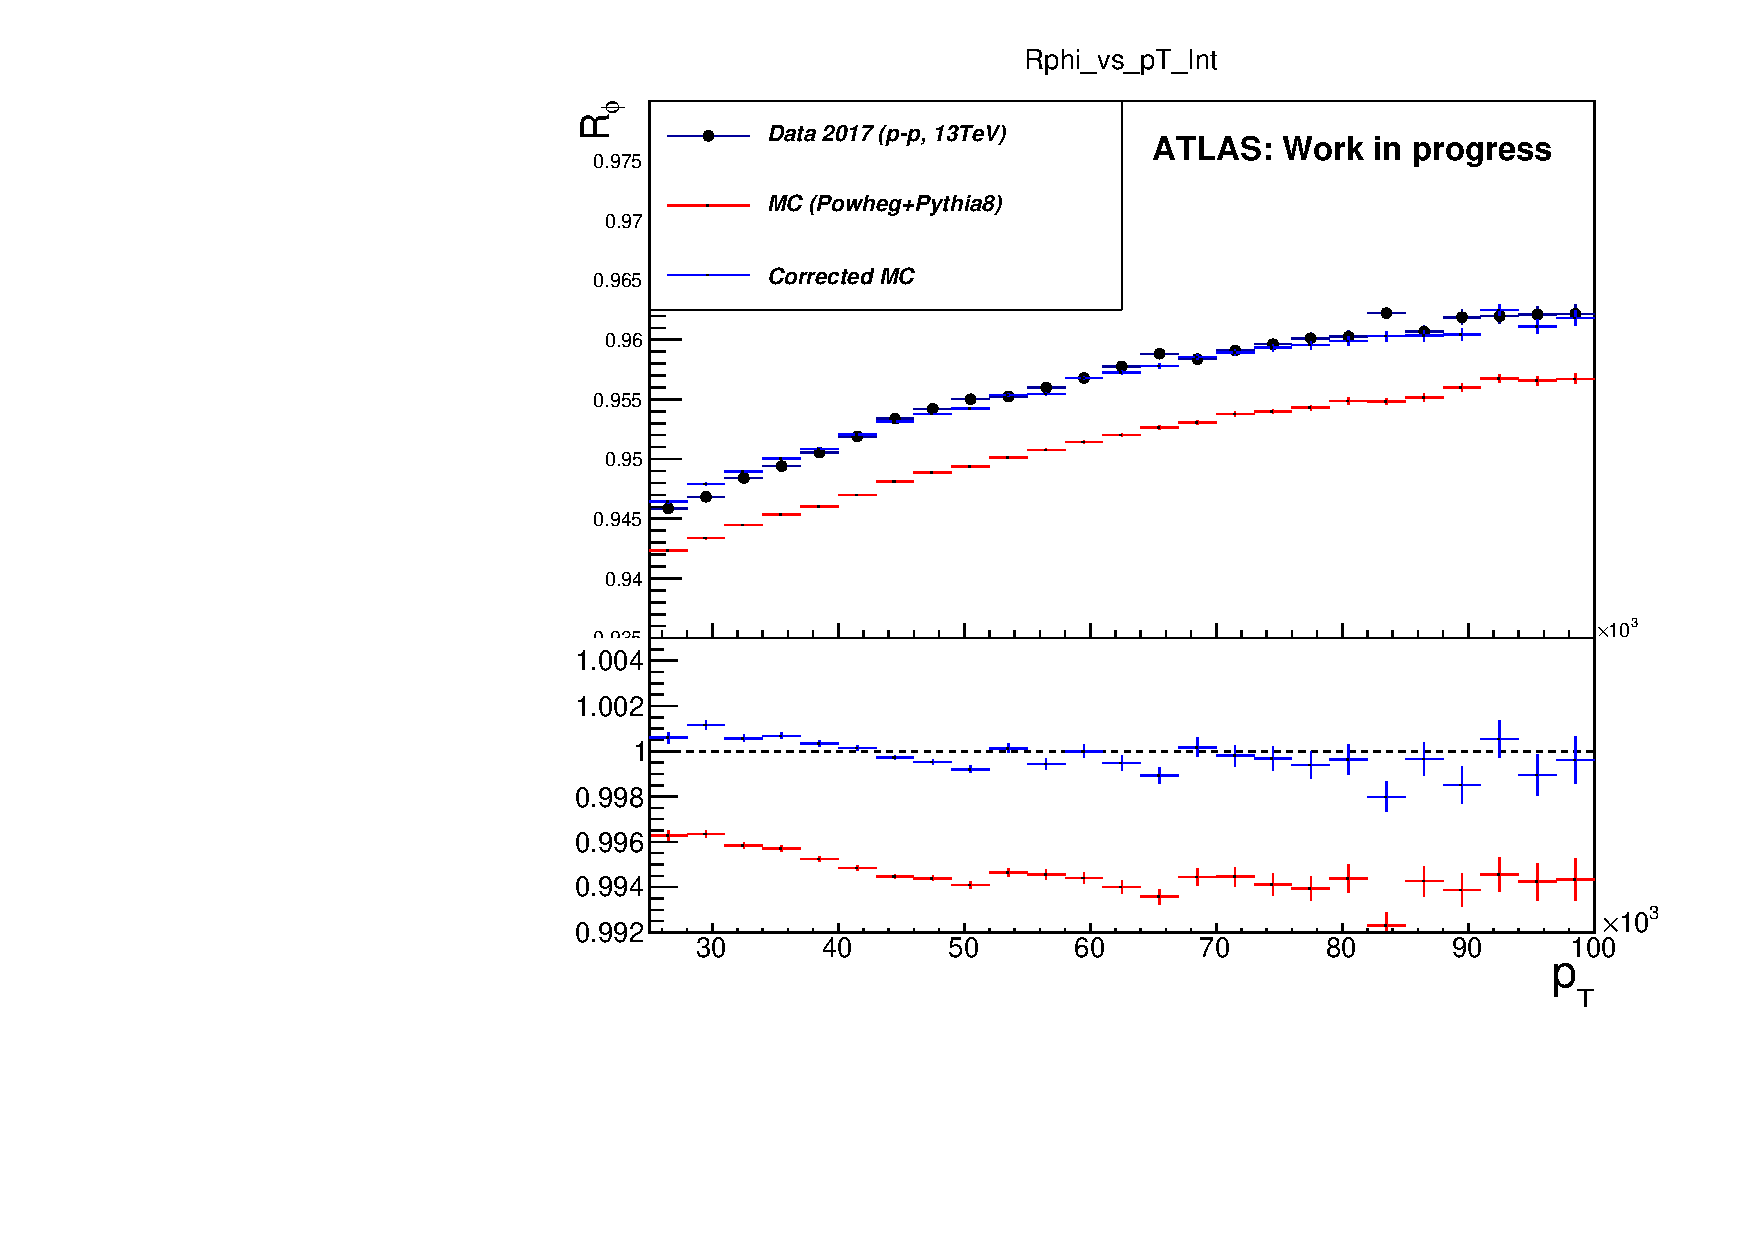
\includegraphics[%
  width=7cm,
  keepaspectratio]{Rphi_vs_pT_Int.pdf}
\caption{Reweighted  $R_{\phi}$ vs $p_T$ integrated over $\eta$.}
\label{Rphi_vs_pT_Int}
\end{figure}
\begin{figure}[htbp]
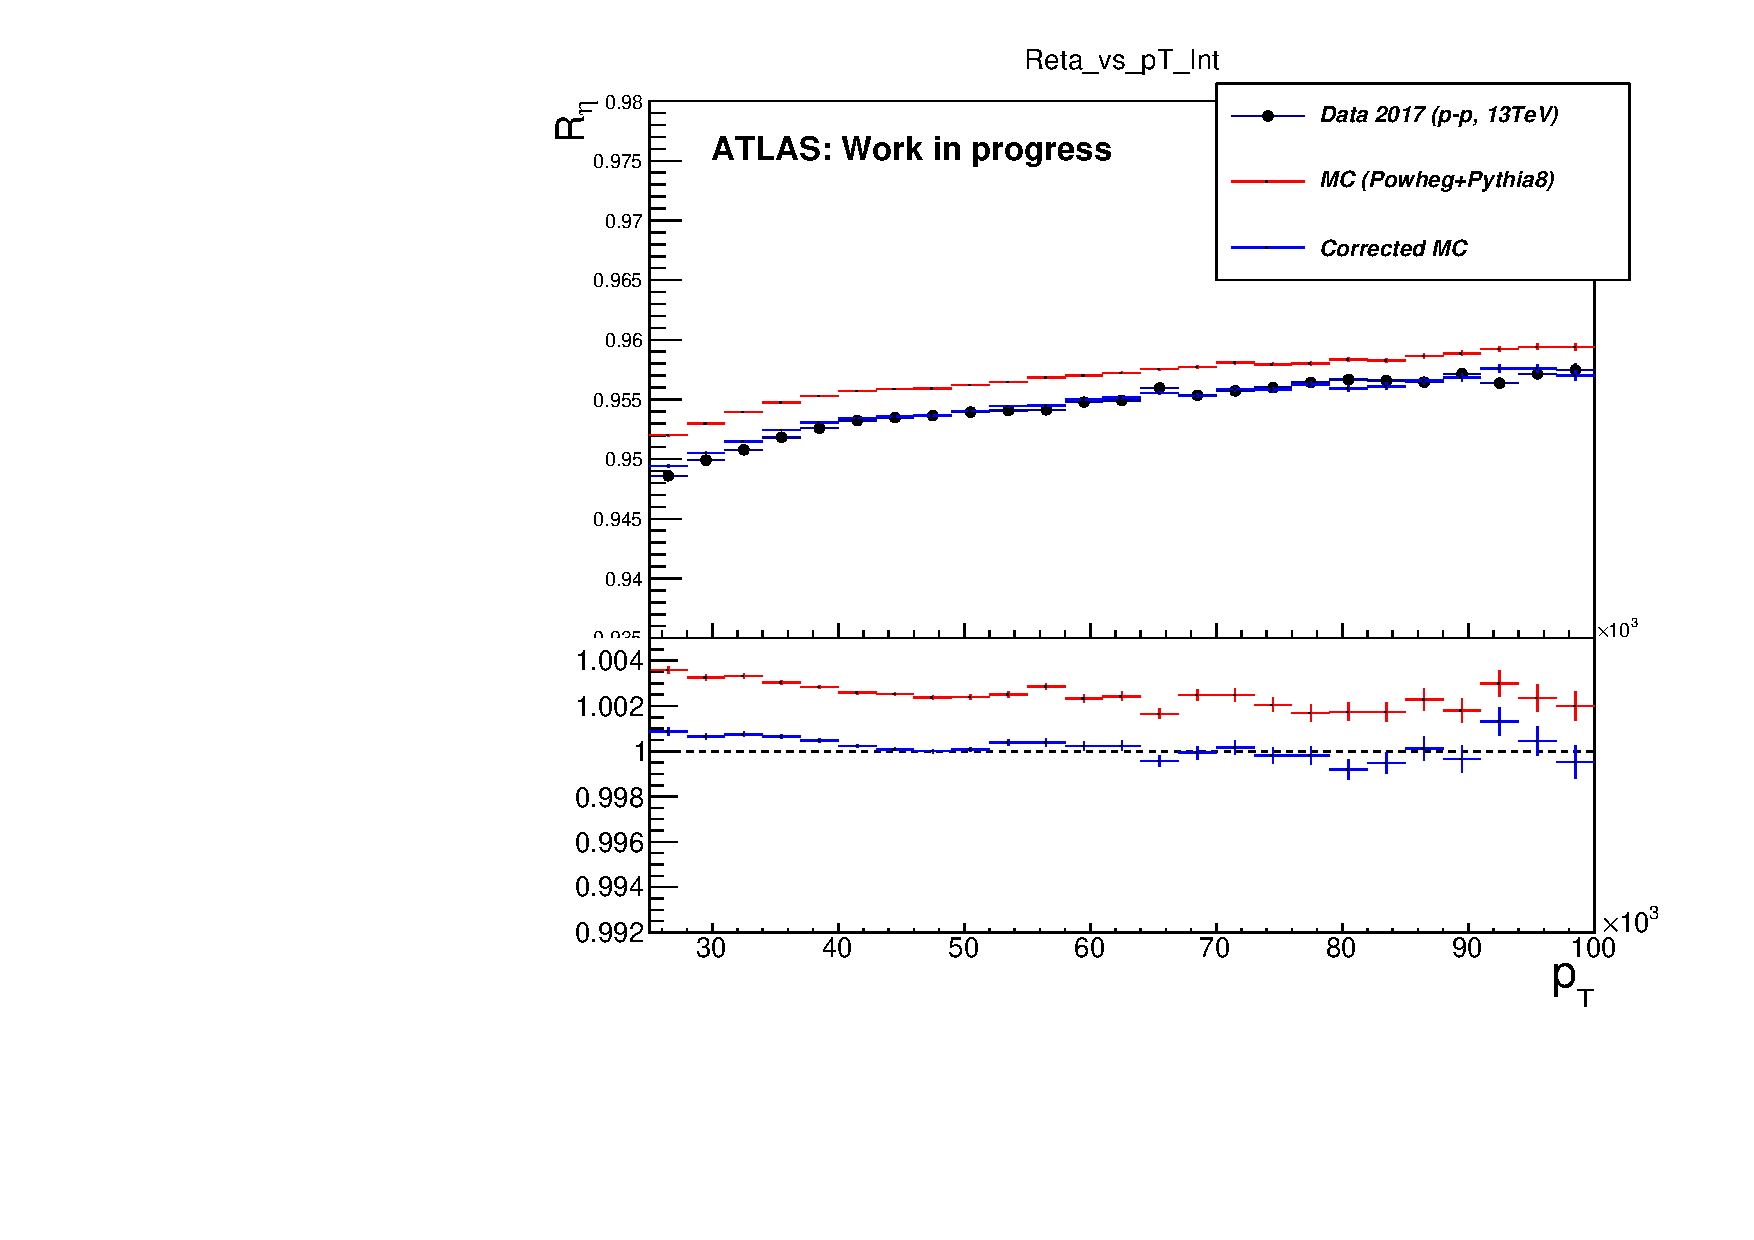
\includegraphics[%
  width=7cm,
  keepaspectratio]{Reta_vs_pT_Int.pdf}
\caption{Reweighted  $R_{\eta}$ vs $p_T$ integrated over $\eta$.}
\label{Reta_vs_pT_Int}
\end{figure}
\begin{figure}[htbp]
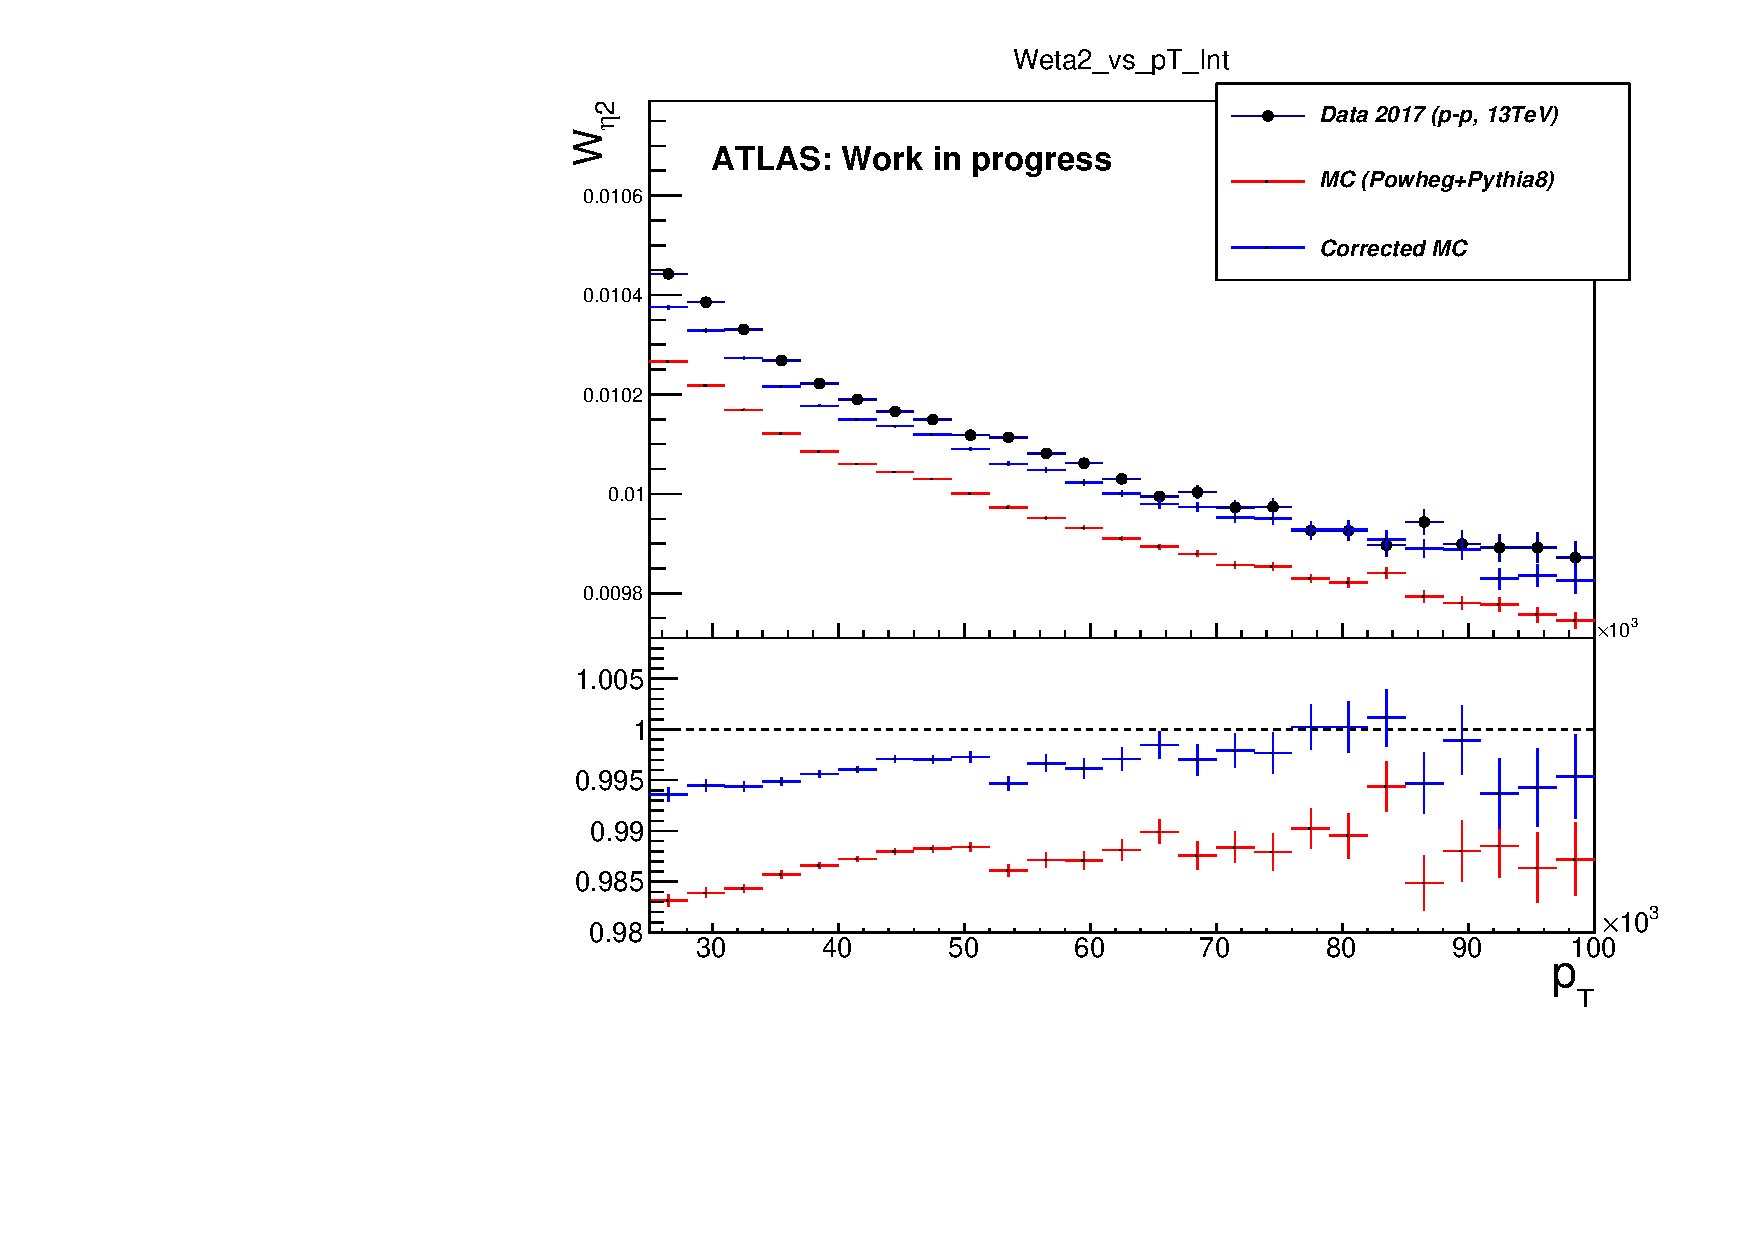
\includegraphics[%
  width=7cm,
  keepaspectratio]{Weta2_vs_pT_Int.pdf}
\caption{Reweighted  $W_{\eta 2}$ vs $p_T$ integrated over $\eta$.}
\label{Weta2_vs_pT_Int}
\end{figure}


\begin{figure}[htbp]
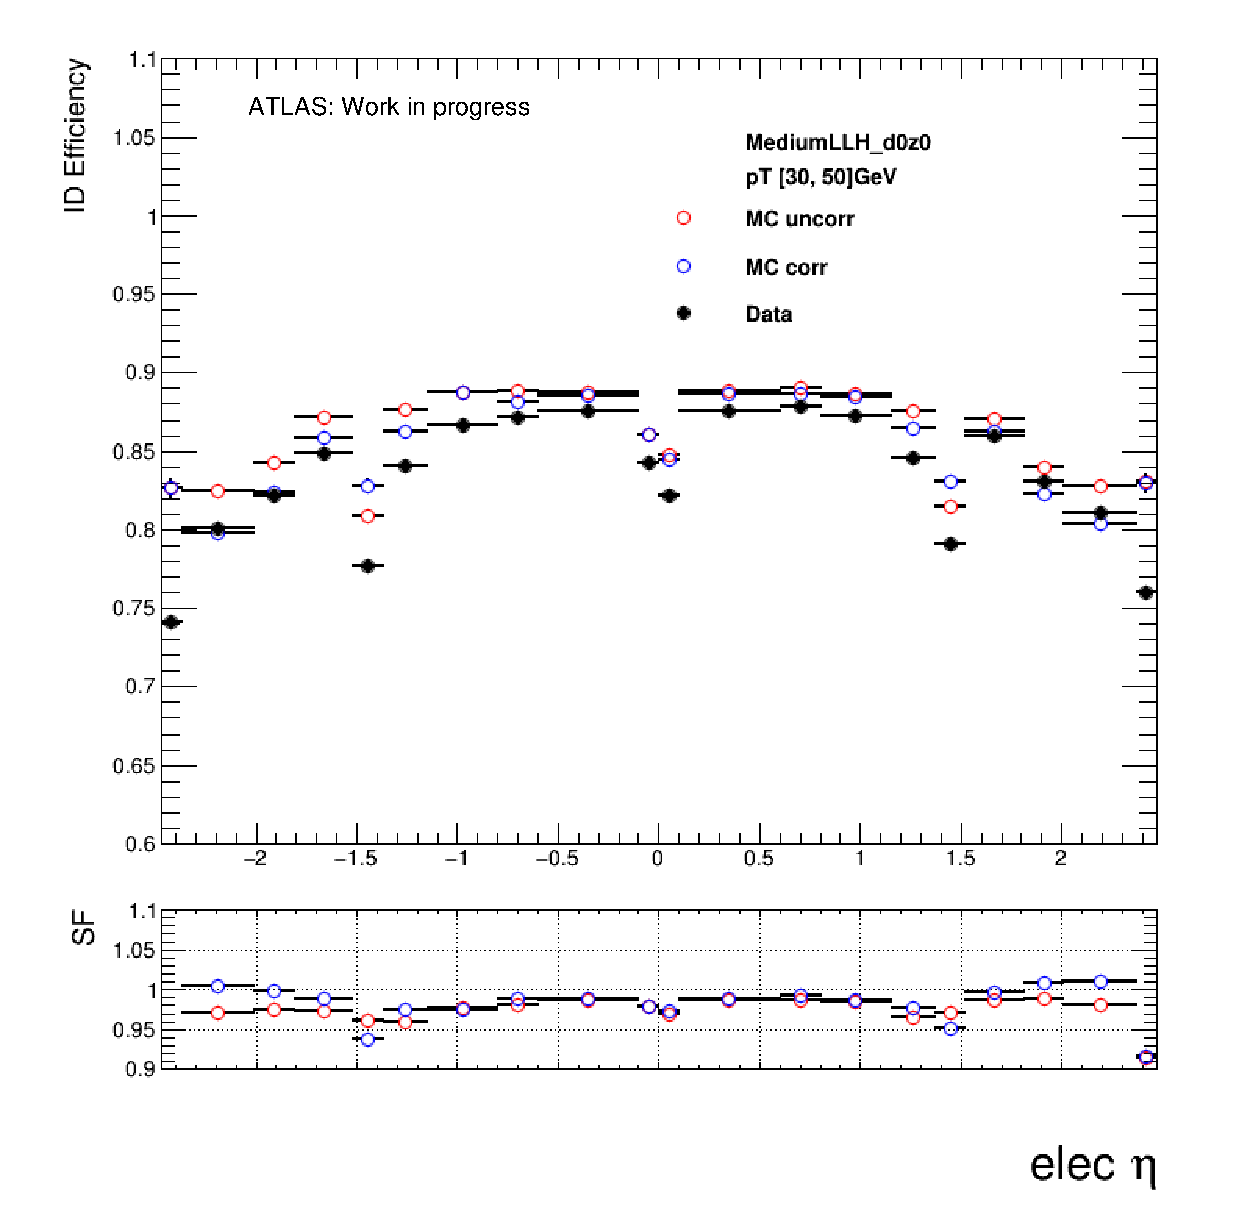
\includegraphics[%
  width=7cm,
  keepaspectratio]{MCeffm247tom237.pdf}\\
\caption{Electron identification efficiency as a function of the electron pseudo-rapidity}
\label{SF}
\end{figure}


\begin{thebibliography}{2}
\bibitem{TDR} ATLAS Collaboration, The ATLAS Experiment at the CERN Large Hadron Collider, JINST 3 (2008) S08003.
\bibitem{RecoID2011} ATLAS Collaboration, Electron reconstruction and identification efficiency measurements with the ATLAS detector using the 2011 LHC proton-proton collision data,
Eur. Phys. J. C 74 (2014) 2941.

\end{thebibliography}

%%% Local Variables:
%%% mode: latex
%%% TeX-master: "~/Documents/adm/jjc05/proceedings/jjc05"
%%% End:
